\section{Human Judgments of Images and World Structure}
\label{sec:human-results}

\subsection{Instrument and Included Responses}
We collected the English visual instrument V01--V11: four image comparisons
and two structure comparisons per respondent, with three short choices per
comparison. The image arm uses preserved maps and two character samples from
seven recorded model configurations on the same promise-city premise. The
structure arm compares full Agora with single-pass generation on ten matched
requests, displaying every authored room, assigned-resident counts, and scene
components in a common containment diagram. These diagrams show world
organization, not movement paths. Source identities are hidden behind A/B
labels; allocation and orientation were fixed before the returns were read.

All eleven PDFs contain eighteen valid choices. Ten also confirm adulthood,
English comprehension, voluntary participation, and no prior development or
detailed-result exposure. V04 leaves all cover confirmations blank and is
excluded pending confirmation, following the released eligibility rule. The
analysis therefore uses ten coded returns, forty image comparisons and twenty
structure comparisons (180 item responses). All 21 image pairs and ten
structure requests retain coverage. This is an exploratory evaluation of fixed
artifacts, not a representative population study. Appendix~\ref{app:human}
documents the questions, exclusions, decoding, and reporting gaps.

\subsection{Structure Preference Does Not Follow Completion}
For each item, a preference for Agora scores 1, a tie 0.5, and a baseline
preference 0; ``Not sure'' is excluded from that item's preference denominator
and reported separately. We average within each request and then equally
across all ten requests, as specified in the released workbook. This prevents
the request receiving four ratings from dominating the overall estimate.

\begin{table}[t]
\centering\small
\setlength{\tabcolsep}{3.2pt}
\begin{tabularx}{\columnwidth}{@{}Yrrrrr@{}}
\toprule
Item & Full & Base & Tie & ? & Score \\
\midrule
Explore & 7 & 13 & 0 & 0 & 40.0\% \\
Clarity & 8 & 11 & 1 & 0 & 32.5\% \\
Scene fit & 7 & 12 & 0 & 1 & 37.5\% \\
\bottomrule
\end{tabularx}

\caption{Structure judgments from ten eligible returns. Full and Base denote Agora
and the single-pass baseline, irrespective of randomized A/B labels; ? = Not
sure. Counts pool twenty comparisons per item. Score is Agora's
\emph{equal-request} mean, not a pooled vote fraction.
No population superiority is inferred from these small counts.}
\label{tab:human-structure}
\end{table}

Respondents select the baseline in thirteen of twenty exploration choices,
versus seven for Agora. Agora's equal-request preference is 40.0\% for
exploration, 32.5\% for world clarity, and 37.5\% for place--scene fit
(Table~\ref{tab:human-structure}). These observations do not support a human
preference advantage for the full pipeline on the displayed structures,
despite its higher completion rate in the construction study. The pipeline's
additional generation cost therefore cannot be justified by a claimed
preference gain from this study.

The pattern varies by request (Figure~\ref{fig:human-structure}). Both Tidal
raters prefer Agora for exploration. All four Clockwork raters prefer the
baseline for exploration while choosing Agora for clarity. Understandability
and desire to explore are thus distinguishable judgments in these returns;
we do not sum them into a single quality score. One or two raters on most
requests cannot identify why a design was preferred, and the diagram omits
institutions, social behavior, and actual play. Equal-compute generation and
interactive evaluation remain separate open tests.

\begin{figure*}[t]
\centering
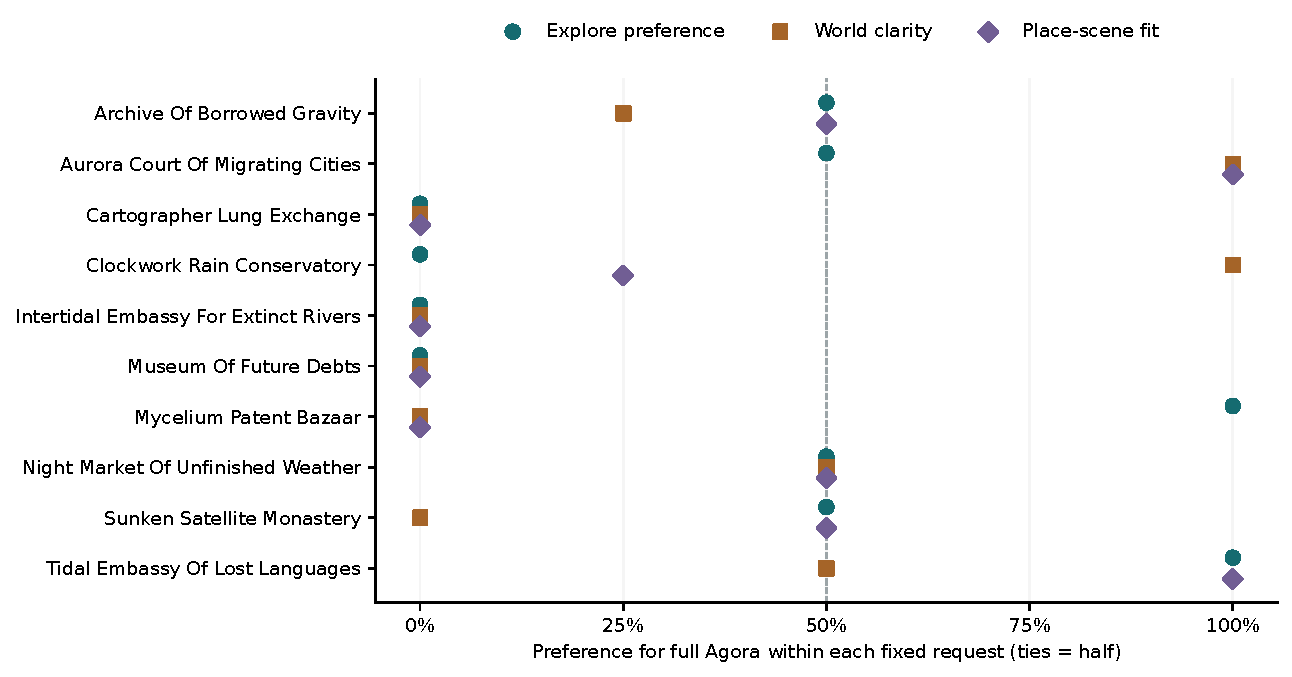
\includegraphics[width=\textwidth]{figures/human_structure_preferences.pdf}
\caption{\paneltitle{World structure: preferences vary by request and item.}
Each point is the fraction favoring full Agora for one request and question,
with a half vote for a tie. The analysis includes 20 comparisons: seven
requests have two raters, two have one, and Clockwork has four. For Tidal
scene fit, one of two raters selects Not sure. These are descriptive fixed-
artifact scores; the dashed line marks equal preference, not a significance
threshold.}
\label{fig:human-structure}
\end{figure*}

\subsection{Image Preference Is Item-Specific}
Figure~\ref{fig:human-images} reports all exact model pairs for exploration,
map readability, and character--world fit. Each model name denotes the
recorded world-generation configuration; the pipeline uses a shared image
generator, so the comparison does not isolate an LLM's ability to render
pixels. Only one prompt has matched archived images.

The three criteria give different outcomes. Both raters prefer the GPT-5.6
Sol artifact to Gemini 3.5 Flash Lite for map readability, but both prefer
the latter for exploration and character fit. The pairwise matrix preserves
these distinctions instead of collapsing them into a single model ranking.
Across the image arm there is one readability tie, one character-fit tie,
and two character-fit abstentions. Four pairs now have one rater, sixteen
have two, and one has four. This sparse, single-scene sample supports
inspection of these particular outputs, not a stable ordering of model
families or general claims about visual quality.

\begin{figure*}[t]
\centering
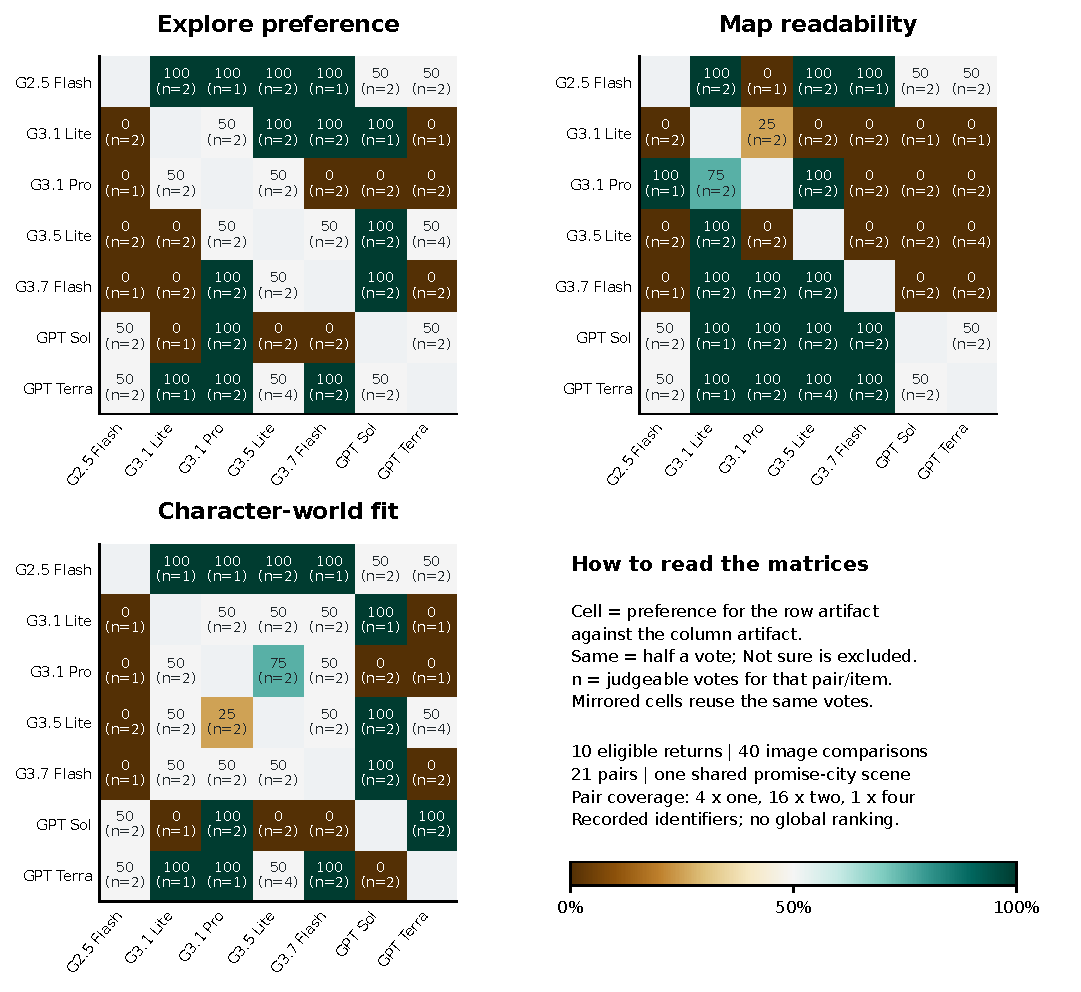
\includegraphics[width=\textwidth]{figures/human_image_preferences.pdf}
\caption{\paneltitle{Images: all 21 pairs, with separate evaluation criteria.}
Cells report the percentage preferring the row artifact over the column
artifact, counting ties as half votes; $n$ is the number of judgeable votes.
Not sure is outside the denominator. Mirrored cells describe the same
comparisons, not additional observations. All outputs share one promise-city
premise and the image pipeline; labels abbreviate archived backend identifiers.
Exact counts, including abstentions, are in Appendix~\ref{app:human}.}
\label{fig:human-images}
\end{figure*}
